\documentclass[UTF8,a4paper]{paper}
\usepackage{ctex}
\usepackage[utf8]{inputenc}
\usepackage{amsmath}
\usepackage{amssymb}
\usepackage{amstext} 
\usepackage{pdfpages}
\usepackage{graphicx}
\usepackage{wrapfig}
\usepackage{listings}
\usepackage{multicol}
\usepackage{float}
\newcommand{\tabincell}[2]{\begin{tabular}{@{}#1@{}}#2\end{tabular}}
\title{第三次书面作业}
\author{张蔚桐\ 2015011493\ 自55}
\begin {document}
\maketitle
\section{}
\begin{multicols}{2}
\subsection{}
显然S边界仅有一个元素,可以看出S边界如图\ref{f1}所示,$S=\{4\le x \le 6;3 \le y \ge 5\}$
\begin{figure}[H]
\centering
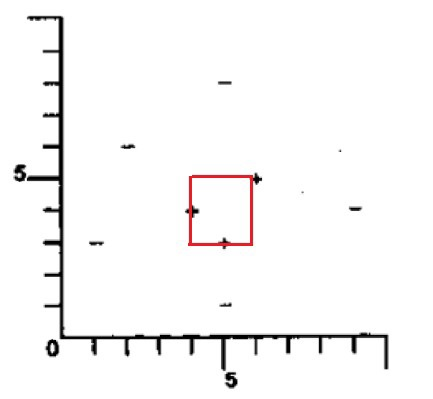
\includegraphics[width=\columnwidth]{1.jpg}
\caption{S边界的唯一假设位置}
\label{f1}
\end{figure}
\subsection{}
显然G边界仅有一个元素,可以看出G边界如图\ref{f2}所示,$G=\{3\le x \le 8;2 \le y \ge 7\}$
\begin{figure}[H]
\centering
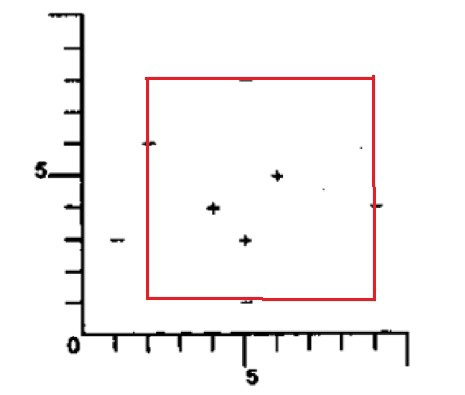
\includegraphics[width=\columnwidth]{2.jpg}
\caption{G边界的唯一假设位置(应为内含的最大矩形边界)}
\label{f2}
\end{figure}
\end{multicols}
\subsection{}
保证能减小变形空间的位置(3,4),不能保证的查询(0,0)(如果为反例则变形空间不变,如果为正例变形空间变空)
\subsection{}
完全学习目标概念要求G和S边界重合,而G边界由反例确定,四个个反例(如果位置合适)可以由边界确定一个G空间,而两个正例可以对角线的确定一个S边界。因此最少需要六个点就可以确定,这六个点有两个正例(3,2),(5,9)以及四个反例(分别在外边界上)

以上正例的位置还可以取为另一侧对角线。

\section{}
不妨我们认为假设空间中的每一项均是对实例空间所有可能的正例的析取,则显然变形空间中的每一个假设对已经出现的正例判1,对已经出现的反例判0,对没有出现的实例x,如果存在一个假设判1,则必然存在另一个合理的假设判0,使得不违背上面的两条要求。因此变形空间中必然有半数的假设将x划为正例,半数将x划为反例。

\section{}
我们采取线性方法学习器,设目标函数为$\hat{y}=a_1x_1+a_2x_2-b$其中$x_1$为身高值,$x_2$为体重值。使得在$\hat{y}$为正时判为男生,为负时判为女生。并且尽可能实现大间隔分类器以提高可推广性。

然而,实际上$x_1$和$x_2$并不在一个分布中,因此我们需要用$\frac{x-\mu}{\sigma}$的方式对分布进行标准化,得到如表\ref{t1}所示的结果

\begin{table}
\centering
\caption{标准化之后的结果}
\label{t1}
\begin{tabular}{|c|c|c|c|}
\hline
编号 & 性别 & $x_1'$ & $x_2'$ \\
\hline 
1 & 男 & -0.35355 & 0.132264 \\
2 & 男 & 0.707011 & 0.473271 \\
3 & 男 & 1.59099 & 1.606062 \\
4 & 女 & -1.59099 & -1.4549 \\
5 & 女 & -0.53033 & -1.00143 \\
6 & 女 & 0.176777 & 0.245633\\
\hline
\end{tabular}
\end{table}
我们画出他们的散点图如图\ref{f4}所示,其中红色为女生,蓝色为男生。我们可以看出明显存在一个女生和一个男生使得整体的线性分割变得困难。甚至可能不存在线性分割。因此我们不妨参考SVM的方式引入松弛因子,使得中央部分的男生和女生“尽可能小偏差的分错”,我们采用的分类面可以取中间两者的中垂线,

最终表达式为$$\hat{y} = x_1+33.3x_2-2253$$

得到男生的值分别为-16,83.25,416.3,女生的值为-482.98,-349.72,16.62,忽略两个干扰样本分类清晰良好。同时我们也可以看出身高因素对分类的影响相对较小。将分类面偏置稍稍移动可以使得两个干扰中的一个男生(或女生)被分类正确。

改进措施:增加样本个数,或采取非线性方式拟合,但因为样本数量太少,只能采取线性拟合。而且不能排除干扰。
\begin{figure}
\centering
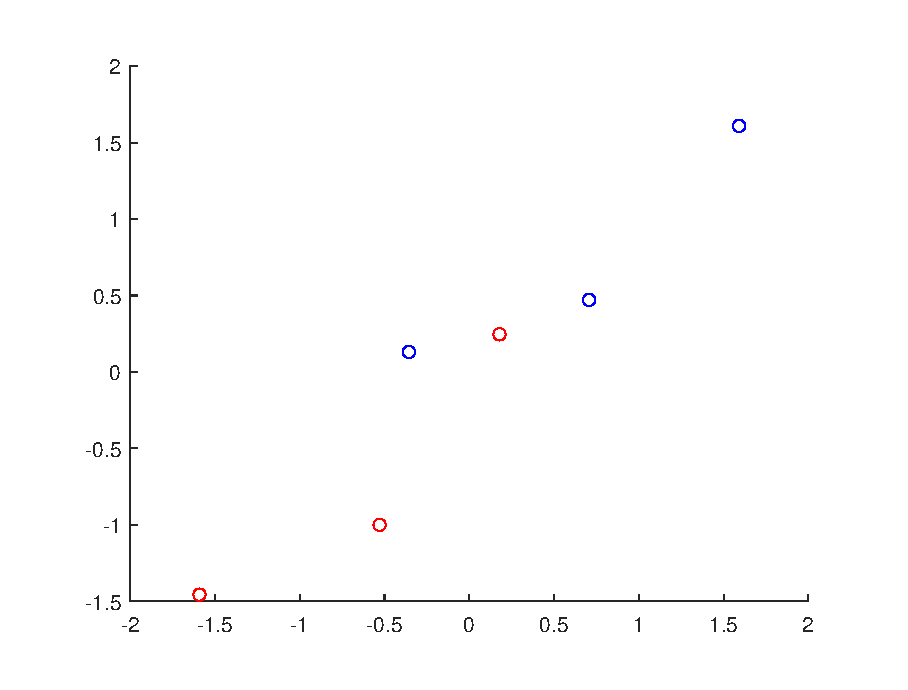
\includegraphics[width=\textwidth]{1.eps}
\caption{散点图}
\label{f4}
\end{figure}
\section{}
\subsection{}
$$S = -0.5\log_2 0.5-0.5\log_2 0.5 =1$$
\subsection{}
$$S = -\frac{2}{3}( -0.5\log_2 0.5-0.5\log_2 0.5)-\frac{1}{3}( -0.5\log_2 0.5-0.5\log_2 0.5)=1$$
没有信息增益
\subsection{}
对a1:
$$S = -0.5(\frac{2}{3}\log_2\frac{2}{3}+\frac{1}{3}\log_2\frac{1}{3})-0.5(\frac{2}{3}\log_2\frac{2}{3}+\frac{1}{3}\log_2\frac{1}{3})$$
$$S = -\frac{2}{3}\log_2\frac{2}{3}+\frac{1}{3}\log_2\frac{1}{3}=-0.9183$$
信息增益0.0817
先分a2,再分a1,得到效果如图\ref{f3}所示
\begin{figure}[H]
\centering
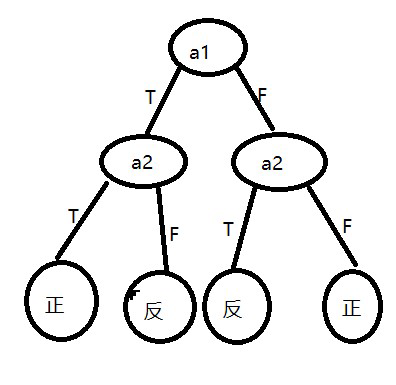
\includegraphics[width=\columnwidth]{3.jpg}
\caption{决策树}
\label{f3}
\end{figure}
\end{document}